\chapter{Technology Review}
This chapter, will discuss the technology used in the projects stack on a theoretical level, detailing features of each piece of technology used in this project.

\section{React}
According to stackoverflow \cite{StackOverflowSurvey}, react.js is the second most common technology for making web based applications at 42.62\%. React was originally launched in May 29 2013, a common misconception is that react is a framework, this is not true, as react is a massive library in which a programmer can make interfaces that revolve around react components \cite{boduch2020react} this along with other features aids to rapid development of a application. React uses the command, create react app to make the application into a framework. React has a seamless development time, making it easier to get applications running using this technology aiding to its popularity over the years \cite{saundariya2021webapp}.

\subsection{React Redux}
The project itself lends a great deal of logic from the redux library of react. These two technologies work very well together and normally go hand in hand \cite{nelson2019developing}. Redux is widely used in this application when state must be changed dynamically without the user noting the change, this greatly supports making a single page application \cite{jadhav2015single}. Redux is best summarized in its key concepts which are employed in the application \cite{caspers2017react}.

\subsubsection{Store}
Store in redux is where the state is stored, this state is then obtained from the store using the getState method, after which the state can be use with the useDisptach method to forward actions.

\subsubsection{Actions}
Actions are responsible for sending the data into the Redux store, actions are the data which alert the store that the state has changed in the application. Redux actions must be a type object, and have other key data so as they are distinguishable to the reducers.

\subsubsection{Reducers}
Redux reducers are viewed as clear functions, such functions take the preceding state and action, then making them inputs thereby returning a new state. A redux reducer script can also be seen as finite state machine, operating on switch statements to switch the state depending on the redux action \cite{holmstedt2019analyzing}.

\subsubsection{Asynchronous Actions}
Lastly redux employs asynchronous actions which can fetch the data from the back-end using redux thunk, after which a response can be handled, and a action can be dispatched so as to update the state of the application. Thunk itself is a middleware, that greatly aids in processing the necessary requests.

\section{Node.js}
Node is a JavaScript run time environment, some of its biggest features include allowing programmers to code in JavaScript on the server side of their application, node can be employed across platforms regardless of OS, and enables programmers to make use of asynchronous programming, so as developers can handle multiple requests in their applications \cite{Node.jsAboutPage}\cite{saundariya2021webapp}. Moreover applications can be launched readily and quickly due to node.js package manager (NPM), greatly aiding a developer to create a application in quick schedule \cite{rawat2020reactjs}. 

\subsection{Node.js Asynchronous Programming}
As eluded to above, Node.js offers asynchronous programming as one of its mainstay features. Such a feature enables a node server to be event driven, and lock free I/O, aiding node in being able to deal with concurrency effectively. Node is able to parse all requests made to it, thereby handling requests in a concurrent fashion using the space execution memory available to it in its one threaded makeup \cite{chhetri2016comparative}.
\begin{figure}[h!]
    \centering
    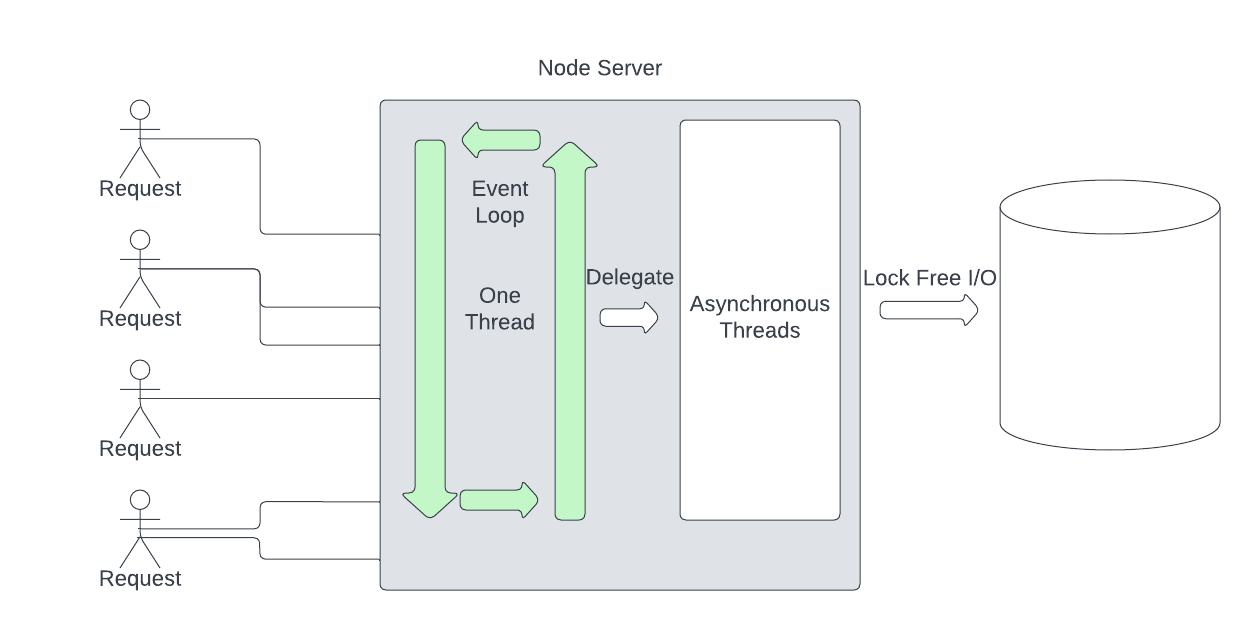
\includegraphics[width=0.8\textwidth]{images/SingleThread.png}
    \caption{Node server makeup using on thread}
    \label{image:SingleThread}
\end{figure}

\subsection{Axios}
Node interacts with react at the front end via HTTP request response, axios helps to streamline this relationship by acting as middleware between node and react, allowing both to send HTTP requests or responses between the server and client sides \cite{saundariya2021webapp}\cite{rawat2020reactjs}.

\section{Express}
Express is a node framework which lends in creating web application, express is normally used in conjecture with node, and can be installed in a application using NPM. Express itself provides an abundance of features for example routing middleware or HTTP capabilities \cite{mardan2018using}.

\subsection{Express as middleware}
Express as a middleware sits between the client and the server, in order to handle request and responses. Express uses functions to take in a request, thereafter such request functions will send back a response, errors when unsuccessful, or relevant data if successful \cite{roomexpress}. In the code snippet below, express is used to log a request and the url to the console. The app.use() method is called, indexing the middleware function, logrequest() is indexed to app.use(), meaning this method will be executed at every incoming request \cite{ExpressMiddleware}. 
\begin{figure}[h!]
    \centering
    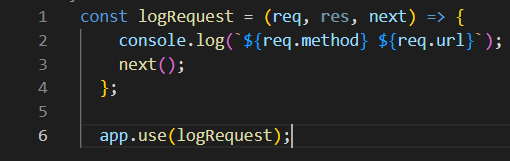
\includegraphics[width=0.4\textwidth]{images/express.png}
    \caption{A brief look at express as a middleware}
    \label{image:express}
\end{figure}
\newline
In the project application of this dissertation an example of how express is used, is to create a request response for users signing into the application.

\subsection{RESTful Express}
Express supports building RESTful APIs for web applications, ways in which Express promotes RESTful usage are, keeping the client side and the server side separate, implementing design patterns for developing web APIs such as aiding in identifying functions to be called for usage, for example get, post, or put. Express can then manipulate such resources over HTTP \cite{REST}, helping to develop an application to be REST compliant by providing robust APIs for handling HTTP requests and responses. Furthermore express promotes REST by handling errors when they occur, or by stating how a user will receive data.

\subsection{Express with HTTP}
Express is built on node.js, using http to access all http functionality, for example get, post being the most common. Express uses http to listen then respond to front end requests \cite{ExpressRouting}. The above-mentioned features allows developers to handle http request through express in the way they see fit, based on the URL and method call, these points make express ideal for making web applications quickly and efficiently.

\section{MongoDB}
Originally developed in 2009, MongoDB is a open source document orientated, NoSQL database which stores, retrieves and manages data for applications \cite{abramova2013nosql}. MongoDB is adeptly suited for numerous applications, for example blog sites which tend to produce a lot of unstructured data, in this case MongoDB is better equipped in dealing with such data in comparison to a RDBMS \cite{agrawal2015survey}. It can be seen as human readable as it stores documents in a JSON like format \cite{calccada2019evaluation}. MongoDB prides itself on having easy to use interfaces, and being able to bring hugely adaptable databases to an application. Beside the features mentioned above, MongoDB ensures acid compliance in their database systems guarantying the validity of data, and uses map reduce as a feature \cite{agrawal2015survey}, which is a data processing model that lends itself to executing actions on sizeable data collections and then assisting in the aggregation of results.

\subsection{MongoDB a NoSQL Database}
There are three types of NoSQL databases, one of which is a document store, MongoDB falls into this category. Document-stored databases are classified as a collection of key-value stores that are then converted into documents and stored in the database \cite{calccada2019evaluation}. One of NoSQL's key features is being able to handle unstructured data to great effect, this is given its rise to popularity in recent years \cite{agrawal2015survey}. Where NoSQL differs from the conventional RDBMS, is that MongoDB's schema is not established in place when compared to a RDBMS, MongoDB will use ID keys in order to retrieve data, as each piece of data is assigned a unique ID key. In reference to the aforementioned, a read/write can only be preformed using the ID key assigned \cite{gyHorodi2015comparative}.

\section{Coding Languages \& Markup Languages}
The below technologies represent the coding languages used in the creation and development of the application.

\subsection{JavaScript}
Developed in 1995, JavaScript or sometimes known as just js, originally created for Netscape 2, although after some time js was preferentially used by Mozilla where it was used to develop web capabilities for Firefox \cite{HistoryJS}. JavaScript is a interpreted language i.e for the computer to understand js, it needs to be complied into something it can understand, normally executable byte code \cite{wilton2004beginning}. With the aforementioned in mind, JavaScript code is interpreted at run time, it is not complied before run time, like for example Java. Attributing to the above, JavaScript is dynamically typed, variables will be assigned at run time, this differs from static typed languages where variables are known at compile time \cite{richards2010analysis}. As such for creating web systems, when a application is running locally, changes can be made to the JavaScript code, then the changes will be shown immediately on the application, provided there are no errors in the code.

\subsection{JavaScript an object orientated language?}
JavaScript is a object orientated language however, js is used more as object based, rather than upholding the principles of object orientated programming. JavaScript as a language promotes the use of being able to change or being agile, as the above mentions js is weakly typed, interpreted, and variables could be removed or added at run time \cite{theisen2019programming}. While js is a object orientated language it is normally not used in such a way, TypeScript a offshoot of JavaScript, is popularly used to adhere with oop principles, which in of itself is a superset of JavaScript.

\subsection{TypeScript}
TypeScript is a superset of JavaScript, this means that TypeScript can understand all JavaScripts syntax and capabilities \cite{cherny2019programming}. TypeScript does more to uphold the principles of object orientated programming, by bringing in classes, interfaces, and is statically typed \cite{bierman2014understanding} catching errors before run time, in many ways TypeScript looks at what JavaScript doesn't do well, then adding features to JavaScript to aid developers. TypeScript does not have a interpreter, instead it compiles to JavaScript as browsers cannot understand TypeScript \cite{jansen2016typescript}. With the above facts in mind, TypeScript is normally used now in favour of JavaScript, as if a person learning web development for the first time, TypeScript uses classes more frequently, and it statically typed language making it more familiar to new comers when compared to JavaScript. Moreover it can be used quite avidly by programmers who use JavaScript as TypeScript understands JavaScript, as it only adds to JavaScript features.

\subsection{TypeScript vs JavaScript}
Below, is a code snippet of TypeScript as a class vs JavaScript as a class, as shown below TypeScript has variables brought in before the constructor i.e variables are known before run time, when compared to JavaScript the variables let person = new Person("Alice", 30); are only assigned during run time.
\begin{figure}[ht]
\begin{minipage}[b]{0.5\linewidth}
    \centering
    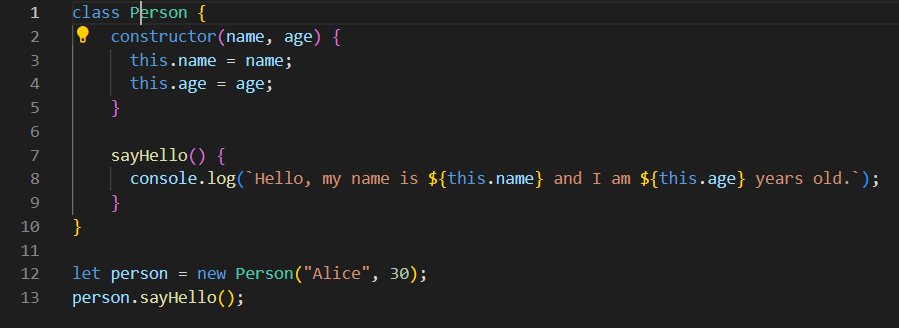
\includegraphics[width=\linewidth]{images/JavaScript}
    \caption{JavaScript as a class}
\end{minipage}
    \hspace{0.5cm}
    \begin{minipage}[b]{0.5\linewidth}
    \centering
   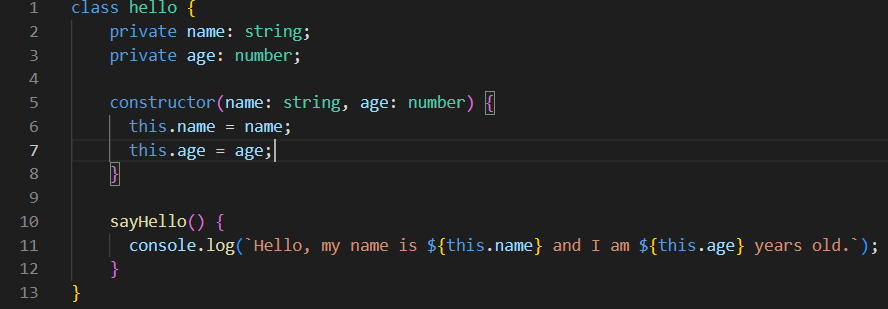
\includegraphics[width=\linewidth]{images/TypeScript}
    \caption{TypeScript as a class}
\end{minipage}
\end{figure}

\subsection{JSX}
JavaScript syntax extension or JSX, which like TypeScript is a addendum to the already established JavaScript. JSX allows developers to outline Reacts object structure into syntax that is comparable to HTML. Simply put JSX, is an XML related addition, allowing programmers to write JavaScript that can appear as a HTML like, and then have it returned as a component in React
\cite{JSX}.

\subsection{HTML}
Hyper Text Markup Language (HTML) is a markup language which is used in representation of web applications. HTML is crucial in any web development as it details the architecture of a web application i.e it explains how the application should be rendered, however the application need not be written in HTML, as it is unable to write functions or carry out complex tasks when compared to JavaScript \cite{minnick2020responsive}.

\subsection{CSS \& Material-UI}
Cascading Style Sheets (CSS) can be closely aligned with the use of HTML or other markup languages, CSS like HTML is also used in changing how a web application is presented, although unlike HTML, CSS tells the application what color, layout or general style elements of the web page should be using \cite{geneves2012analysis}. The creation of pleasing designs can be employed quickly using a CSS framework Material-UI, which follows googles material design patterns, Material-UI comes with existing React components, for example SVG icons, uniformity in displaying forms or navigation bars, and other features. Material-UI can help developers worry less about the look of a application when compared to using normal CSS, as Material-UI will handle most of the aesthetic of the application \cite{nguyen2022building}.

\subsection{JSON}
JavaScript Object Notation, allows programs to represent JavaScript objects in plain text, JSON is used to serialize and parse objects over the network, normally between the front end and the back end. However this comes at a price as the plain text used, are much larger in size when compared to their binary equivalent, therefore parsing must be preformed on both sides for example in client side and server side \cite{JSON}.

\subsubsection{JSON Web Token}
Web tokens are used to identify if users are verified on certain systems for instance, if a user signed into Facebook, a web token would be assigned to them, asserting a authenticated user \cite{JWT}. A JSON web token uses a JSON object to assert safety between two parties normally the user and the client or application the user wishes to use \cite{jones2015json}. Authorization is the most regular use of a JSON web token, when a user is logged into Facebook for example, they will then be able to avail of the activities which Facebook advertises, using their JSON web token which is stored in local storage, all of which is hidden from the users view \cite{JWT}.

\section{Cypress}
Cypress automation test tool is a relatively new web automation tool only being released in 2017. Cypress is a client side testing tool created for web applications, Cypress greatly encourages Behaviour Driven Development, building tests side by side while creating a web application, then asserting such tests pass as development advances \cite{WhyCypress}.

\subsection{Cypress Architecture}
Cypress is often contrasted with Selenium, although the two testing tools are architecturally different. Cypress is built using Node.js, and comes in its own npm module to be installed locally, then running npm to open cypress in a browser window in order to open the application the developer wishes to test \cite{taky2021automated}. Altering web traffic at will, is how Cypress performs operations at the network layer. This gives Cypress the opportunity to change what goes into and out of the browser, allowing Cypress to also adjust code that could cause glitch's or errors in the browser's automation \cite{WhyCypress}, resulting in a smother testing experience, enabling the engineer to obtain accordant outcomes \cite{pelivani2022comparative}. As Cypress is installed into a developers local machine using node, it allows the automation to use the local operating system in order to make use of the camera for taking screenshots of failing or passing tests, and recording videos of the automated test suite.
\begin{figure}[h!]
    \centering
    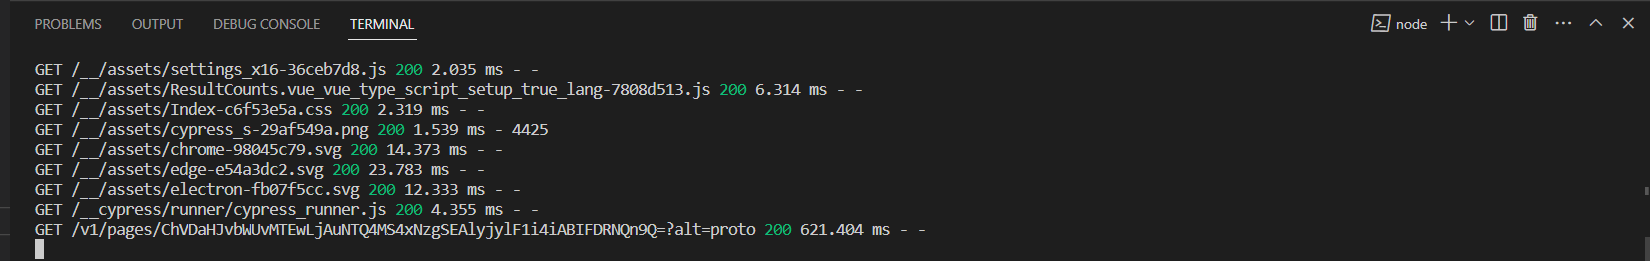
\includegraphics[width=0.8\textwidth]{images/CypressAndNode.png}
    \caption{Node running the server side for Cypress}
    \label{image:CypressAndNode}
\end{figure}
\begin{figure}[h!]
    \centering
    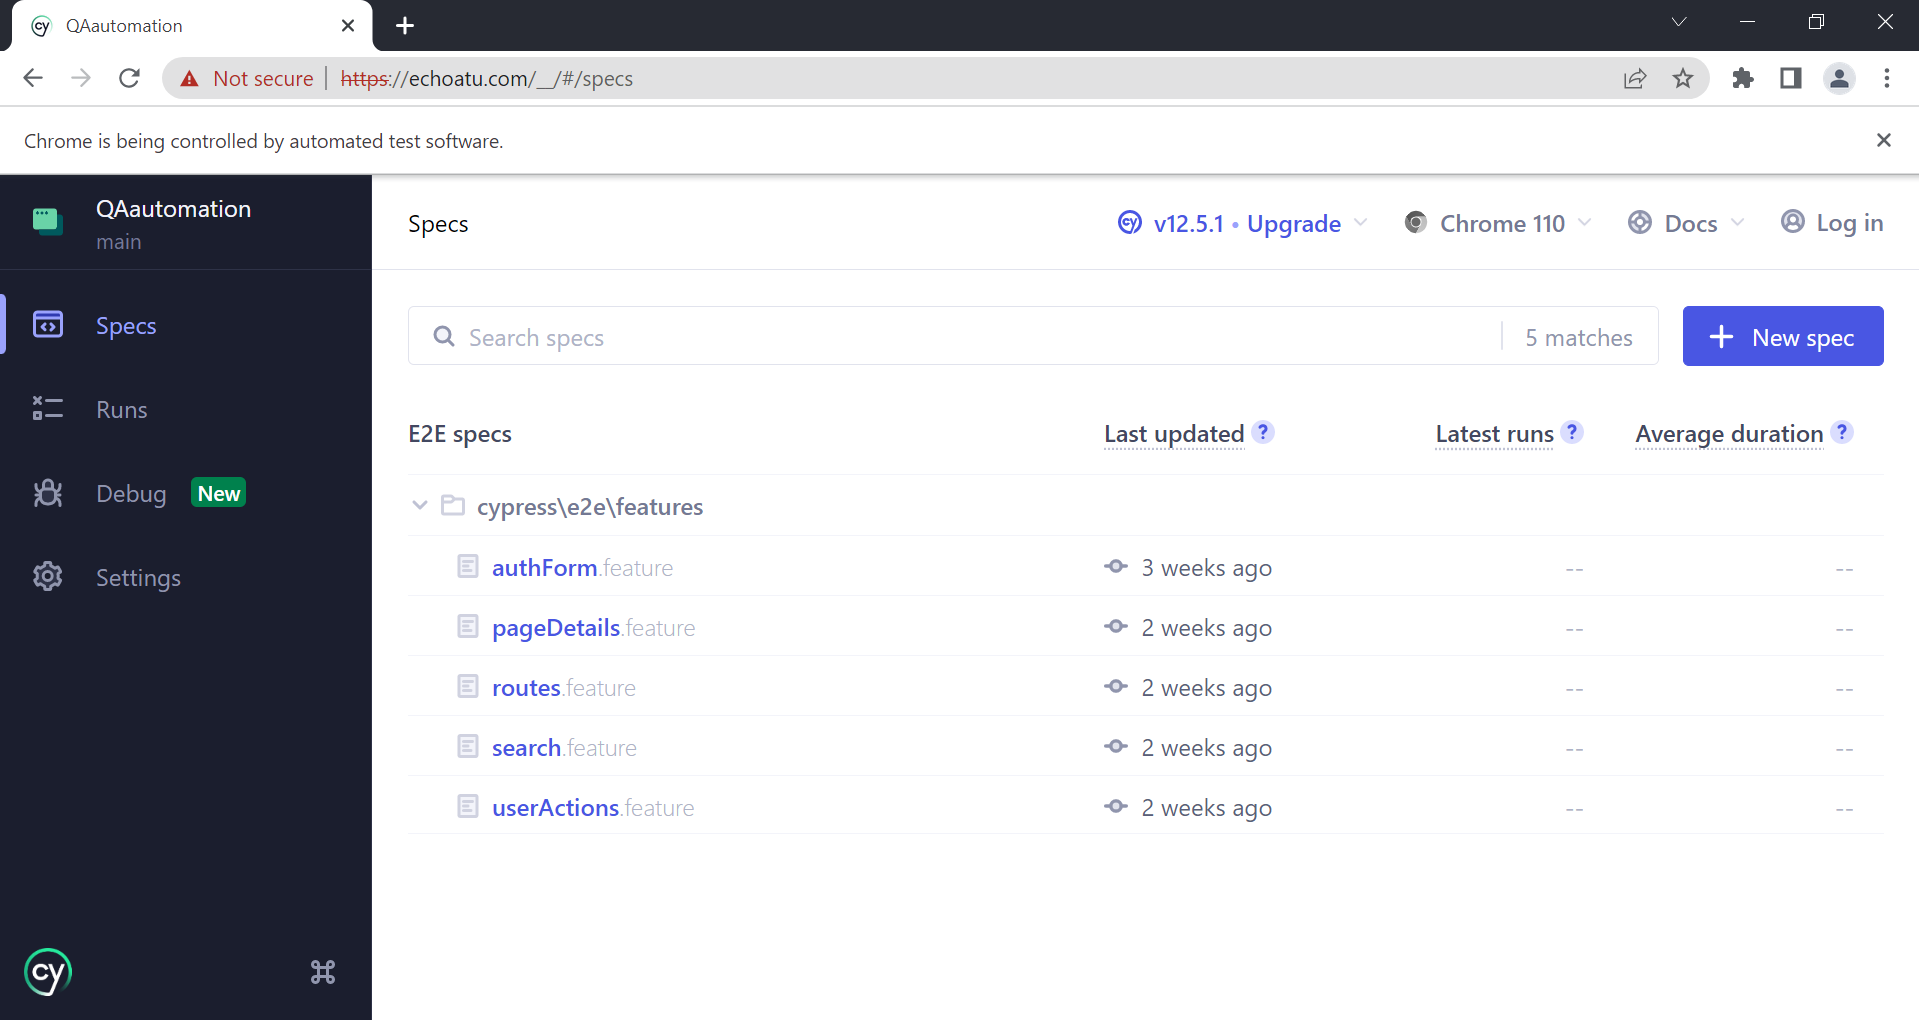
\includegraphics[width=0.5\textwidth]{images/BrowserCypress.png}
    \caption{Cypress running in the browser supported by node.js}
    \label{image:BrowserCypress}
\end{figure}

\subsection{Cypress Features}
Cypress contains a number of capabilities for example Cypress uses the wait command at will in order to wait for the DOM to load in correctly, this is needed greatly as Cypress tests sometimes preform blindingly fast, although if a test engineer wishes for extra time to be applied the cy.wait command can be hard coded in \cite{SwitchCy}. JavaScript is the predominate coding language used in Cypresses testing framework, and in turn this means TypeScript too is greatly used in Cypress, considering many web applications are made in the aforementioned languages \cite{MostUsedLang}, this makes for a easy learning curve from Front End developer to test engineer and vice versa. Further traits that Cypress contains as testing capabilities are, the ability to use multiple browsers other than chrome for example Microsoft edge, Firefox, or electron, using Cypress dashboard to detect flaky tests i.e tests which passed but then began to fail, the tester can begin to pinpoint a flaky test and update the test in order to make it more reliable \cite{WhyCypress}.

\subsection{Cypress \& Cucumber}\label{sec:cypress-cucumber}
Cypress can be further integrated, to use behavior driven development (BDD) with the aid of a tool called Cucumber.

\subsubsection{Cucumber}
Cucumber as mentioned above is a framework which buttresses BDD, Cucumber enables the user to create tests in gherkin syntax of which gherkin syntax is normal text which make up features \cite{pelivani2022comparative}. The aforementioned features consists of various steps which Cucumber must work through in order to assert if the test is passing, or failing. Then the plain text is linked to step definitions, which is the coding section of Cucumber, thereafter the written code carries out the task assigned using the gherkin syntax e.g Then The echo should be deleted \cite{Cucumber}.

\begin{figure}[ht]
\begin{minipage}[b]{0.5\linewidth}
    \centering
    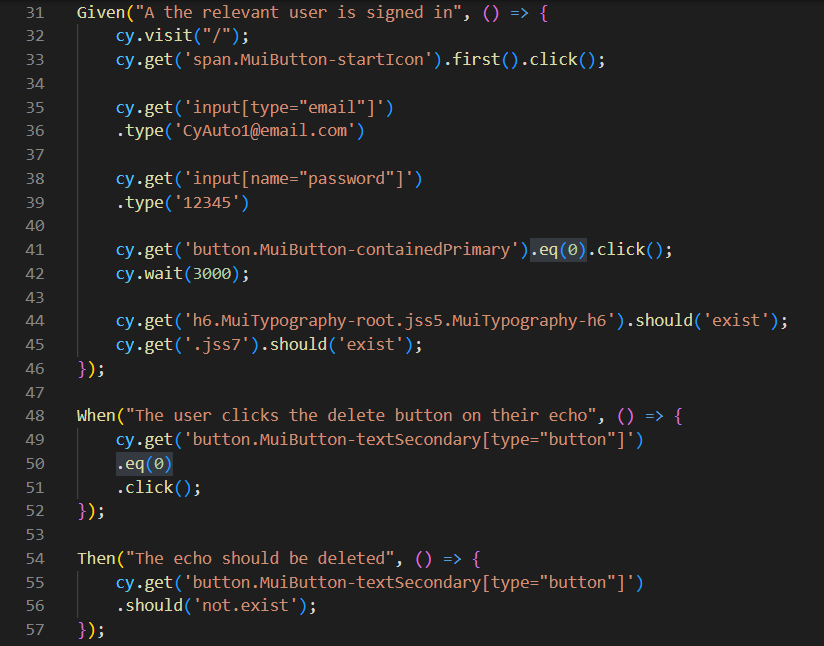
\includegraphics[width=\linewidth]{images/StepDefination}
    \caption{Step Definition}
    \label{image:StepDefination}
\end{minipage}
    \hspace{0.5cm}
    \begin{minipage}[b]{0.5\linewidth}
    \centering
   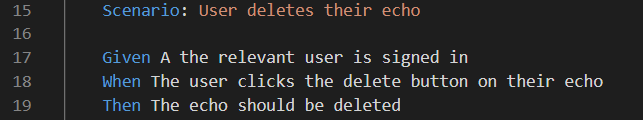
\includegraphics[width=\linewidth]{images/Feature}
    \caption{Gherkin Feature}
    \label{image:Feature}
\end{minipage}
\end{figure}

\newpage
\subsubsection{Cucumber integration with Cypress}
Cucumber is not installed with Cypress, thus it has to be installed in order to access gherkin syntax, and have it incorporated with Cypress. After Cypress is installed, Cucumber can further be added to the testing file by using these commands in the CLI, npm i @badeball/cypress-cucumber-preprocessor, this package allows programmers to define Gherkin syntax in running their Cypress tests \cite{cypress-cucumber-preprocessor}\cite{CypressPlugins}. Now Cucumber should is installed, Cypress should work using Gherkin syntax after changes to the configuration file \cite{IntergratingCucumber}.

\section{Jira Software}
Jira Software was originally created in 2002, it is a tool used by software development teams in order to track the amount of work done. Jira supports many agile methodologies which attribute as to the why it is used so widely in industry, it promotes change and ability to alter the software project \cite{fisher2013utilizing}. As mentioned above Jira uses the agile perspective to software development, for example test driven development(TDD) in which the software requirements are made into cases before code is developed in the application, thereafter the tests will assert that the application fulfils the users expectation \cite{havazik2020design}. Jira makes the above possible with, team planning where tasks are created outlining the objectives to be done during the sprint, a sprint is a duration of work normally consisting of one or two week iteration, inside the sprint, tasks called stories which are assigned to team members to be completed before the end of the sprint, during the sprint daily stand up meetings are arranged to scale how well each team member are doing with their tasks, after the sprint ends, their is a team review, and a new sprint starts again repeating the process \cite{marques2018assessing}.

\section{Kommunicate}
Kommunicate is a chat bot AI which can help a user if they need to ask questions about the application. A developer can make their own AI bot through kommunicate \cite{Kommunicate}, customize it to suit the needs of their web application, and optimize the AI to answer an questions a user might conceive while visiting the application.

\section{Platform as a Service}
Platform as a service (PaaS) refers to services that enable developers to launch their applications into a cloud-based development environment. PaaS enables an application deployment without the need to worry for operating systems or other infrastructure \cite{keller2010platform}.

\subsection{Heroku}
Heroku is a PaaS that allows developers to deliver applications online without going through the infrastructure set up \cite{WhyHeroku}. Heroku is able to run programmes across the network in virtual repositories, after which are then executed in the browser during run time \cite{danielsson2021heroku}. Such repositories can be scaled up or down based on the developers needs, for most one person projects or simple business applications only one container would be needed. 

\subsection{Hostinger}
Hostinger, another form of PaaS which allows programmers to host sites on a domain. In turn this allows the developer to choose the name of their domain after their application is built. When a developers application is built, simply drag and drop the application from the local drive into the file manager hostinger provides. After which hostinger deals with deployment of the application, then being available on the browser using the domain name that was picked upon registering the application. Features hostinger provides includes, allowing web traffic into the associated domain to exceed bandwidth where hostinger will handle it, domain name can be provided after sign up, HTTP/3 usage, and GIT support are among the most useful \cite{Hostingerfeatures}.